\documentclass[11pt,a4paper]{article}
\usepackage{fontspec}
\usepackage[french]{babel}
\usepackage[a4paper,margin=2.3cm]{geometry}
\usepackage{amsmath,booktabs,tabularx,array,graphicx,caption,subcaption,enumitem,microtype,float}
\usepackage[hidelinks]{hyperref}
\captionsetup{font=small,labelfont=bf}
\setlist{itemsep=1pt,topsep=3pt}
\setlength{\parskip}{3pt}
\graphicspath{{../analyse/figures/}{img/}{../analyse/fiches/}}
\title{\textbf{Anticiper le risque de décrochage scolaire,\\ région par région}\\[4pt]\large Burkina Faso, rentrée 2026/27}
\author{Data Challenge Burkina 2026 · Éducation · Défi 1}
\date{Novembre 2026}

\begin{document}
\maketitle

\begin{abstract}
\noindent Le décrochage scolaire au primaire prend deux formes au Burkina Faso : brutale, quand la violence ferme les écoles et fait chuter les effectifs ; lente, quand une part croissante d'enfants n'achève pas le cycle (51,6\,\% d'achèvement en 2024/25, contre 62,0\,\% en 2021/22). Nous proposons un score de risque de 0 à 100 qui réunit les deux, une alerte qui se précise de septembre à janvier, un facteur dominant par région qui oriente l'action, et un tableau de bord utilisable sans réseau. Tous les modèles sont évalués sur des années qu'ils n'ont pas vues, contre la règle « comme l'an passé ». Pour la rentrée 2026/27, cinq régions sur treize relèvent d'une action immédiate ; elles réunissent environ 184\,700 enfants qui n'atteignent pas le CM2 (63\,\% du pays). Rejouée sur le passé, la règle de priorité aurait désigné 35\,\% des régions et contenu 71\,\% des fortes baisses d'effectifs de l'année suivante.
\end{abstract}

\section{Le besoin}
Avant chaque rentrée, quand se décident les réouvertures, les cantines et les affectations d'enseignants, un décideur pose trois questions : \emph{où agir en premier}, \emph{où la situation va s'aggraver}, et \emph{combien d'enfants sont en jeu}, avec, pour chaque région, \emph{sur quoi agir}.

Les outils existants arrivent trop tard ou voient mal. Le taux d'abandon par cohorte n'est connu qu'après la rentrée suivante et compte comme abandons les élèves déplacés réinscrits ailleurs. Le suivi de l'éducation en situation d'urgence recense les écoles fermées (5\,336 en février 2024) mais pas les élèves qui manquent encore. Les systèmes d'alerte élève par élève supposent un identifiant unique, encore en phase pilote au Burkina.

Trois contraintes ont guidé la conception : des données \textbf{agrégées} par région et par année, sans aucune donnée personnelle ; une alerte disponible \textbf{avant la rentrée} ; un outil \textbf{utilisable sans réseau}, puisque le risque est le plus fort là où la connexion manque.

\section{Les données}
\subsection{Les données du challenge}
Vingt et un tableaux de la DGESS couvrent 2015/16 à 2024/25 pour les \textbf{treize anciennes régions} : effectifs, écoles, nouveaux inscrits, taux de scolarisation, d'admission et d'achèvement, réussite au CEP, par sexe. Ils ne contiennent ni redoublants, ni abandons, ni provinces, ni effectifs par niveau et par région. Le décrochage est donc mesuré par deux signaux observables : la \textbf{chute des effectifs} d'une année sur l'autre et le \textbf{taux d'achèvement} (TAP).

Huit contrôles de cohérence ont été appliqués ; toutes les sommes concordent (garçons et filles, régions et national, statuts, niveaux). Deux anomalies sont signalées : une ligne recopiée au préscolaire en 2019/20, et des taux supérieurs à 100\,\% dans les régions d'accueil, où les projections de population ignorent les déplacements. Les effectifs bruts sont donc plus fiables que les taux.

\subsection{Les sources externes}
\begin{table}[H]\centering\small
\begin{tabularx}{\textwidth}{@{}lXl@{}}\toprule
Source & Apport & Dans le dépôt\\\midrule
ACLED (via HDX) & incidents de violence par province et par mois, 1997--2026 & agrégat (brut non redistribuable)\\
IGB, via OCHA & limites 2025 ; correspondance 13/17 régions, 45/47 provinces & table et carte\\
INSD (cod-ps) & population 2024 par province & brut\\
Cadre harmonisé & population en phase 3 ou plus d'insécurité alimentaire & brut et agrégat\\
EDS 2021 & femmes sans instruction, grossesses précoces & valeurs régionales\\
INSD, EHCVM 2021 & pauvreté par région & tableau recopié\\
CONASUR & personnes déplacées accueillies, fin 2022 & brut et agrégat\\
Insecurity Insight & attaques contre l'éducation & agrégat\\\bottomrule
\end{tabularx}\caption{Sources externes.}\end{table}

Le découpage de 2025 compte dix-sept régions, mais les données du challenge n'en connaissent que treize. L'analyse est conduite sur les treize anciennes régions, présentées sous leur nom de 2025 (par exemple « Goulmou + Sirba + Tapoa » pour l'ancien Est) grâce à la correspondance officielle de l'IGB. Une région scindée en 2025 conserve un seul score.

\section{Ce que montrent les données}
\begin{figure}[H]\centering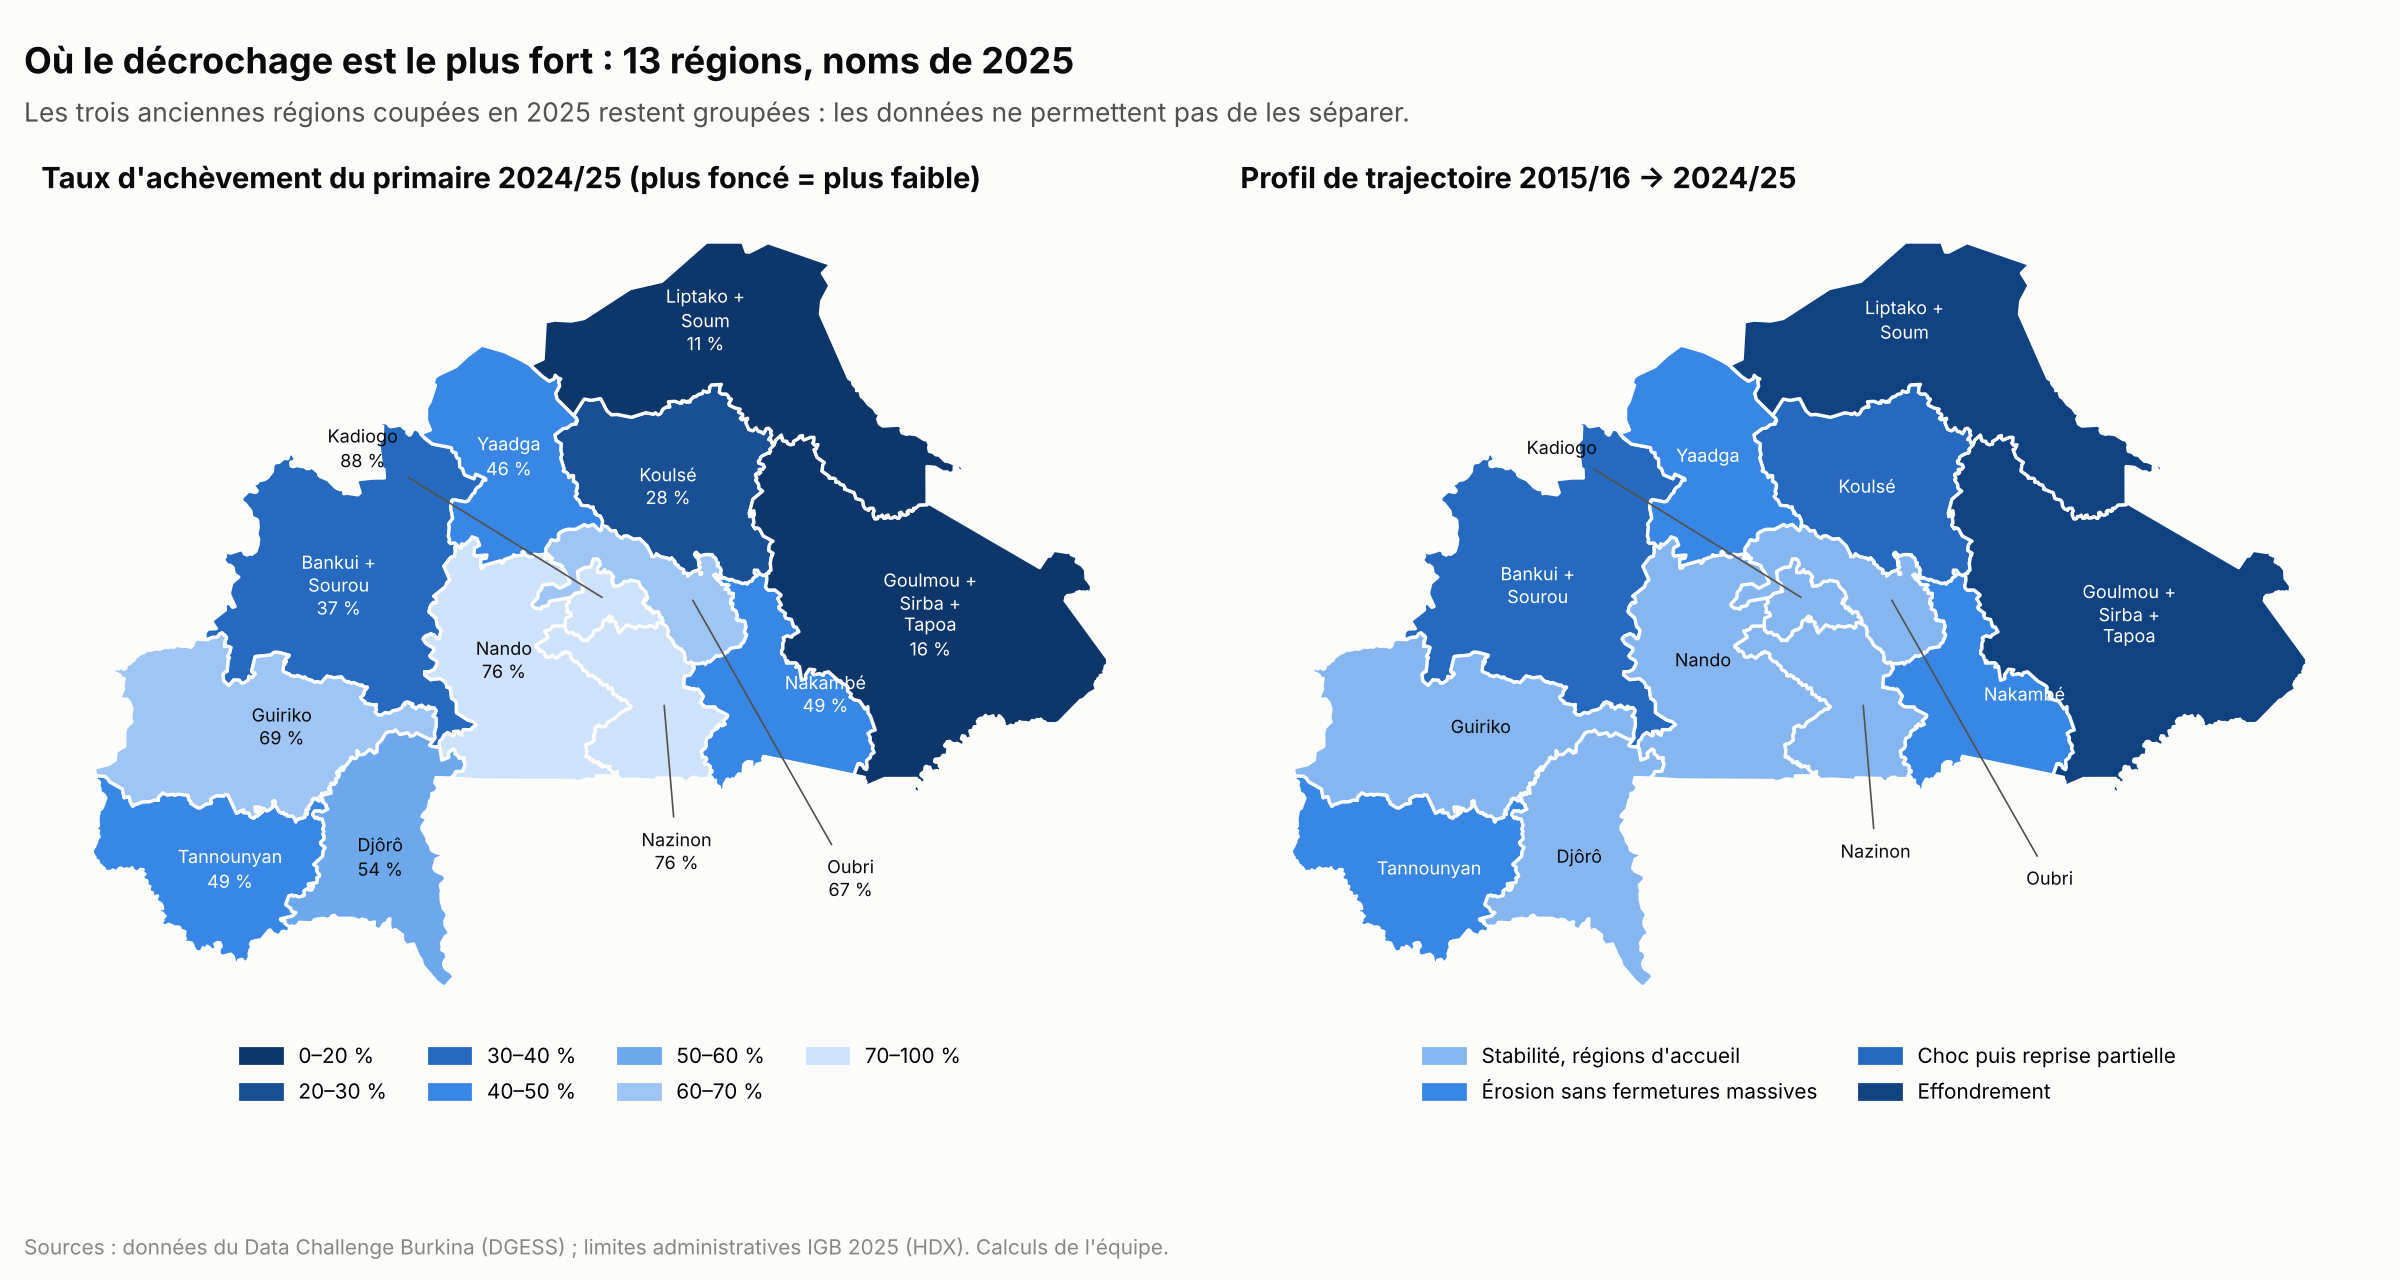
\includegraphics[width=.92\textwidth]{08_carte_profils_achevement.png}
\caption{Taux d'achèvement du primaire en 2024/25 et profils d'évolution des régions.}\end{figure}
\begin{itemize}
\item \textbf{Le choc de 2022/23.} Les effectifs du primaire passent de 3\,174\,946 à 2\,835\,544 ($-10{,}7$\,\%), les écoles de 14\,427 à 12\,780.
\item \textbf{L'entrée repart, l'achèvement s'effondre.} En 2024/25, les effectifs atteignent un record (3\,308\,096), mais l'achèvement tombe à 51,6\,\%, son plus bas de la décennie ; les garçons achèvent moins que les filles (47,7\,\%).
\item \textbf{Les fermetures d'écoles expliquent l'essentiel des variations d'effectifs} : 1\,\% d'écoles en moins correspond à 0,78\,\% d'élèves en moins ($R^2 = 0{,}87$, 117 variations).
\item \textbf{Cinq régions décrochent nettement} : l'Est (achèvement de 40,2\,\% à 16,5\,\%), le Sahel (11,1\,\%), le Centre-Nord, la Boucle du Mouhoun et le Nord. Les régions d'accueil (Centre, Hauts-Bassins, Centre-Ouest, Centre-Sud) se maintiennent.
\item \textbf{Le retard est très persistant} : la corrélation de rang de l'achèvement d'une année à l'autre vaut 0{,}97. La carte d'une année désigne de façon fiable les régions de l'année suivante.
\end{itemize}

\section{Méthode}
Une règle s'applique à tous les modèles : ils sont évalués \textbf{sur des années qu'ils n'ont pas vues}, contre la règle « comme l'an passé », avec une liste de candidats fixée avant les tests.

\subsection{Le risque de chute des effectifs}
On estime pour chaque région la probabilité $p$ que les effectifs du primaire baissent de plus de 5\,\% à la rentrée suivante, à partir des seuls incidents de violence de l'année scolaire écoulée (octobre à septembre), par une régression logistique :
\begin{equation}
z = -5{,}77 + 0{,}98\,\ln(1+I_t) + 0{,}86\,\bigl[\ln(1+I_t) - \ln(1+I_{t-1})\bigr],\qquad p = \frac{1}{1+e^{-z}},
\end{equation}
où $I_t$ est le nombre d'incidents de l'année $t$. Le premier terme mesure le \emph{niveau} de la violence, le second son \emph{escalade} ; le logarithme traduit un effet décroissant. Les trois paramètres sont estimés sur 104 observations (13 régions, 2016/17 à 2023/24), dont 19 fortes baisses.

\paragraph{Exemple.} À Yaadga, $I_t = 250$ et $I_{t-1} = 131$ : $z = -5{,}77 + 0{,}98 \times 5{,}53 + 0{,}86 \times 0{,}64 = 0{,}21$, soit $p = 55$\,\%.

\paragraph{Validation.} Le passé est rejoué année par année : pour prévoir 2019/20, le modèle n'apprend que sur les années antérieures, et ainsi de suite.
\begin{table}[H]\centering\small
\begin{tabular}{@{}lcc@{}}\toprule
Modèle (forte baisse l'année suivante) & AUC & Baisses annoncées\\\midrule
\textbf{Logistique, violence seule (retenu)} & \textbf{0,83} & \textbf{64\,\%}\\
Forêt aléatoire, toutes variables & 0,78 & 64\,\%\\
Logistique, toutes variables & 0,75 & 57\,\%\\
Règle d'escalade simple & 0,68 & 50\,\%\\
Aucun modèle & 0,50 & --\\\bottomrule
\end{tabular}\caption{Performances sur des années non vues. L'AUC est la probabilité que le modèle classe au-dessus une région qui chute face à une région qui ne chute pas.}\end{table}
Les probabilités classent bien les régions mais restent approximatives (score de Brier 0,166 contre 0,169 pour le taux de base) : on lit des niveaux (élevé à partir de 40\,\%, moyen à partir de 15\,\%) plutôt que des pourcentages exacts.

\subsection{Une alerte qui se précise au fil de l'année}
Six signaux plus fins ont été testés à partir des données mensuelles. Deux améliorent l'alerte, et tous deux portent sur le \emph{moment} de la violence : les incidents de juillet à septembre (alerte de septembre, AUC 0{,}85) et ceux d'octobre à décembre (alerte de janvier, AUC 0{,}88), contre 0{,}83 pour le modèle de référence. La part du territoire touchée, la violence des régions voisines et les attaques contre l'éducation n'améliorent pas l'alerte.

\subsection{Le score global}
Le score combine les deux formes de décrochage :
\begin{equation}
\text{score} = 100 \times \Bigl(0{,}5\,p + 0{,}5\,\bigl(1 - \tfrac{\text{TAP}}{100}\bigr)\Bigr),
\end{equation}
où $p$ mesure le décrochage brutal et $1-\text{TAP}/100$ la part d'enfants qui n'achèvent pas le primaire. Les poids sont fixés avant tout test et les bornes sont fixes : le score d'une région ne dépend que de ses propres données. À Yaadga, $p = 0{,}55$ et $\text{TAP} = 46{,}4$\,\%, d'où un score de $50 \times 0{,}55 + 50 \times 0{,}536 = 54$. Les extrêmes sont Goulmou + Sirba + Tapoa (66) et Kadiogo (7).

Rejoué sur 2019/20--2023/24 à nombre de régions égal, le score obtient une AUC de 0{,}80 (0{,}83 pour le risque seul) et repère 64\,\% des fortes baisses et 65\,\% des élèves perdus, contre 71\,\% et 69\,\% pour la matrice de priorité. \textbf{Le score résume, il ne cible pas mieux} : il est affiché comme lecture d'ensemble, et la matrice reste la règle de ciblage.

\subsection{La matrice de priorité}
\begin{table}[H]\centering\small
\begin{tabular}{@{}ll@{}}\toprule
Priorité & Règle\\\midrule
1 -- agir maintenant & achèvement sous la moyenne nationale (51,6\,\%) \emph{et} $p \geq 40$\,\%\\
2 -- veille renforcée & achèvement sous la moyenne \emph{ou} $p \geq 15$\,\%\\
3 -- consolider & autres régions\\\bottomrule
\end{tabular}\caption{Règle de priorité.}\end{table}
Rejouée sur le passé avec la seule information de chaque année, la priorité 1 désignait 35\,\% des régions mais contenait 71\,\% des fortes baisses de l'année suivante et 69\,\% des élèves perdus ; aucune forte baisse n'est tombée en priorité 3.

\subsection{Le facteur dominant}
Pour chaque facteur de fond $f$ et chaque région $r$, on calcule
\begin{equation}
w(r,f) = |\rho_f| \times z_{r,f},
\end{equation}
où $z_{r,f}$ est l'écart de la région à la moyenne des treize, en écarts-types, orienté pour qu'une valeur positive signifie une exposition plus forte, et $|\rho_f|$ la force du lien du facteur avec l'achèvement 2024/25.
\begin{table}[H]\centering\small
\begin{tabular}{@{}lccccccc@{}}\toprule
 & Violence & Mères sans instr. & Déplacés & Faim & Grossesses préc. & Pauvreté & Préscolaire\\\midrule
$|\rho_f|$ & 0,92 & 0,85 & 0,83 & 0,72 & 0,72 & 0,69 & 0,55\\\bottomrule
\end{tabular}\caption{Poids des facteurs de fond.}\end{table}
Le facteur de plus grand poids est le facteur dominant, auquel est associé un levier ; le deuxième indique la suite. La réussite au CEP est écartée en raison d'un effet de sélection. Ce facteur \textbf{explique et oriente l'action, il ne prévoit pas} : ajoutés au modèle de risque, la faim et les facteurs de fond dégradent l'alerte (AUC 0,76 contre 0,82).

\subsection{Le nombre d'élèves}
Les approches qui prévoient les effectifs « à l'aveugle » font toutes moins bien que la règle « comme l'an passé », car elles ne voient pas les réouvertures, qui relèvent de décisions de l'État. Dès que le nombre d'écoles ouvertes à la rentrée est connu, l'erreur est divisée par deux (4{,}2\,\% contre 8{,}6\,\%) :
\begin{equation}
\ln\frac{E_{t+n}}{E_{2024/25}} = 0{,}0197\,n + 0{,}7784\,\ln\frac{O_{t+n}}{O_{2024/25}},
\end{equation}
où $E$ désigne les élèves et $O$ les écoles ouvertes. Le tableau de bord permet de saisir ce nombre sur le terrain, même sans réseau.

\subsection{Ce qui a été testé et écarté}
\begin{itemize}
\item \textbf{L'hypothèse « insécurité $\times$ pauvreté »} : l'interaction n'est pas détectée (effet $+0{,}14$, IC à 95\,\% $[-0{,}38\,;\,+0{,}25]$) et le modèle avec interaction prévoit moins bien (4,46 points d'erreur contre 4,24) ; l'insécurité a en revanche un effet propre ($-1{,}01$ point d'achèvement par unité de log des incidents).
\item \textbf{L'apprentissage automatique} (Ridge, forêt aléatoire, gradient boosting) fait moins bien que « comme l'an passé » sur la variation de l'achèvement (4,54 à 4,79 points contre 4,23).
\item \textbf{La faim} accompagne le recul (+10 points de population en crise alimentaire vont avec environ $-4$ points d'achèvement) mais n'annonce rien de plus que la violence.
\item \textbf{L'achèvement 2025/26} : aucun modèle ne bat « comme l'an passé », qui est donc la prévision affichée, avec une fourchette tirée des erreurs passées.
\end{itemize}

\section{Résultats pour la rentrée 2026/27}
\begin{table}[H]\centering\footnotesize
\begin{tabularx}{\textwidth}{@{}>{\raggedright}p{2.7cm}>{\raggedright}p{2.1cm}cccc>{\raggedright}Xr@{}}\toprule
Région (2025) & Ancienne région & Score & $p$ (\%) & TAP (\%) & Prio. & Agir sur & Hors CM2\tabularnewline\midrule
Goulmou + Sirba + Tapoa & Est & 66 & 49 & 16{,}5 & 1 & l'insécurité & 50\,600 \tabularnewline
Liptako + Soum & Sahel & 65 & 41 & 11{,}1 & 1 & l'accueil des déplacés & 28\,200 \tabularnewline
Koulsé & Centre-Nord & 60 & 48 & 27{,}7 & 1 & les grossesses précoces & 42\,000 \tabularnewline
Yaadga & Nord & 54 & 55 & 46{,}4 & 1 & la pauvreté & 28\,600 \tabularnewline
Bankui + Sourou & Boucle du Mouhoun & 52 & 41 & 37{,}2 & 1 & l'insécurité & 35\,300 \tabularnewline
Nakambé & Centre-Est & 39 & 26 & 48{,}7 & 2 & l'insécurité & 25\,100 \tabularnewline
Tannounyan & Cascades & 27 & 3 & 49{,}4 & 2 & les grossesses précoces & 12\,800 \tabularnewline
Guiriko & Hauts-Bassins & 23 & 15 & 68{,}8 & 2 & (aucun : consolider) & 20\,400 \tabularnewline
Djôrô & Sud-Ouest & 25 & 4 & 53{,}5 & 3 & les grossesses précoces & 11\,800 \tabularnewline
Oubri & Plateau Central & 16 & 0 & 67{,}2 & 3 & (aucun : consolider) & 9\,500 \tabularnewline
Nazinon & Centre-Sud & 15 & 6 & 75{,}5 & 3 & le préscolaire & 5\,500 \tabularnewline
Nando & Centre-Ouest & 14 & 4 & 75{,}9 & 3 & (aucun : consolider) & 11\,900 \tabularnewline
Kadiogo & Centre & 7 & 1 & 87{,}5 & 3 & (aucun : consolider) & 9\,900 \tabularnewline
\bottomrule
\end{tabularx}\caption{Score, risque, achèvement, priorité, facteur dominant et enfants d'environ 11 ans qui n'atteignent pas le CM2 (ordre de grandeur).}\end{table}
\begin{itemize}
\item Les cinq régions en tête du score sont exactement les cinq régions en priorité 1. Elles réunissent environ 184\,700 enfants qui n'atteignent pas le CM2 (63\,\% du pays).
\item Entre le score 2025/26 et la prévision 2026/27, le risque monte à Yaadga (41 $\to$ 54), Koulsé (52 $\to$ 60), Guiriko (17 $\to$ 23), Liptako + Soum (61 $\to$ 65), Nazinon (12 $\to$ 15), Goulmou + Sirba + Tapoa (63 $\to$ 66).
\item Les leviers diffèrent au sein même de la priorité 1 : l'insécurité dans l'Est et la Boucle du Mouhoun, l'accueil des déplacés au Sahel, les grossesses précoces au Centre-Nord, la pauvreté au Nord.
\item L'alerte de septembre porte Yaadga à 61\,\% et Guiriko de 1\,\% à 20\,\% : une région qui tient encore mais où le risque monte, à placer en veille.
\end{itemize}
\begin{figure}[H]\centering
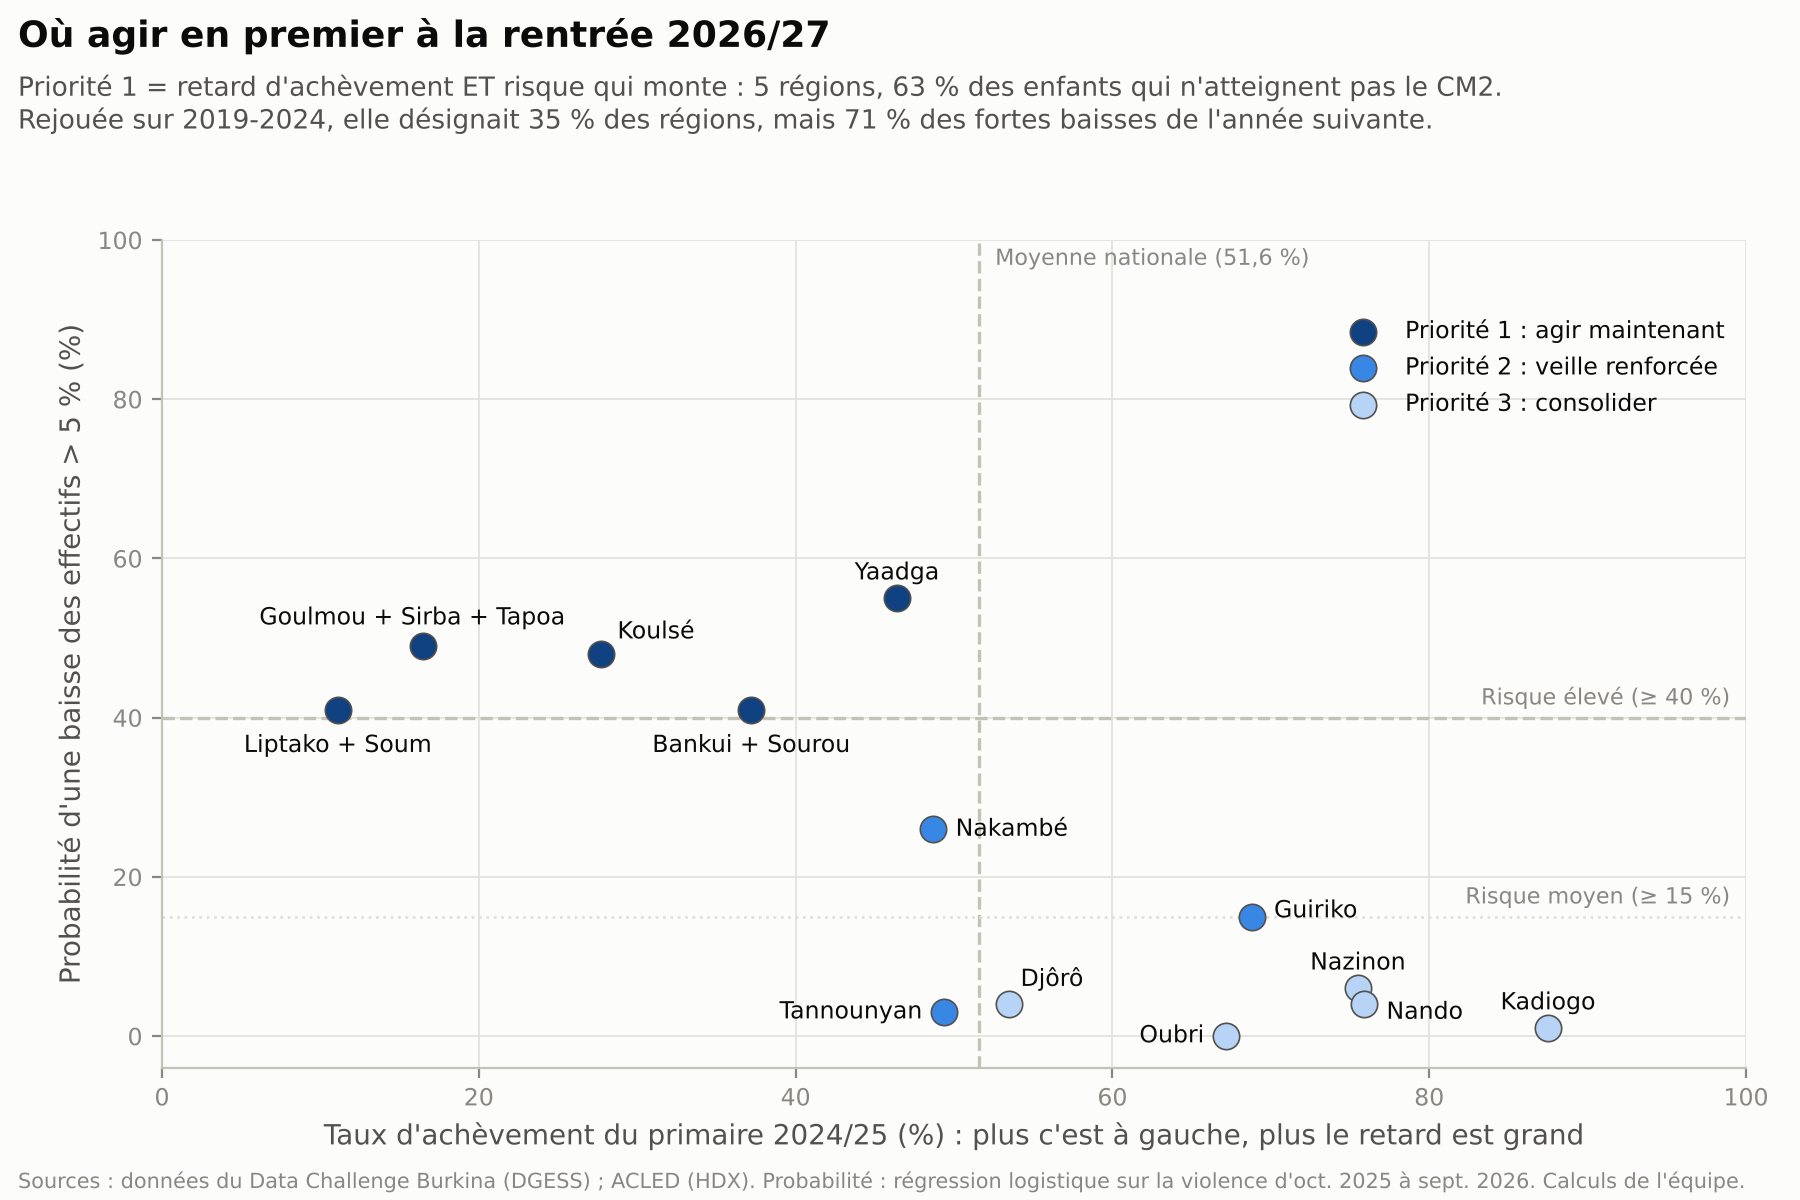
\includegraphics[width=.86\textwidth]{15_matrice_priorite_2026_27.png}
\caption{Matrice de priorité 2026/27 : retard d'achèvement et risque de chute.}\end{figure}
\begin{figure}[H]\centering
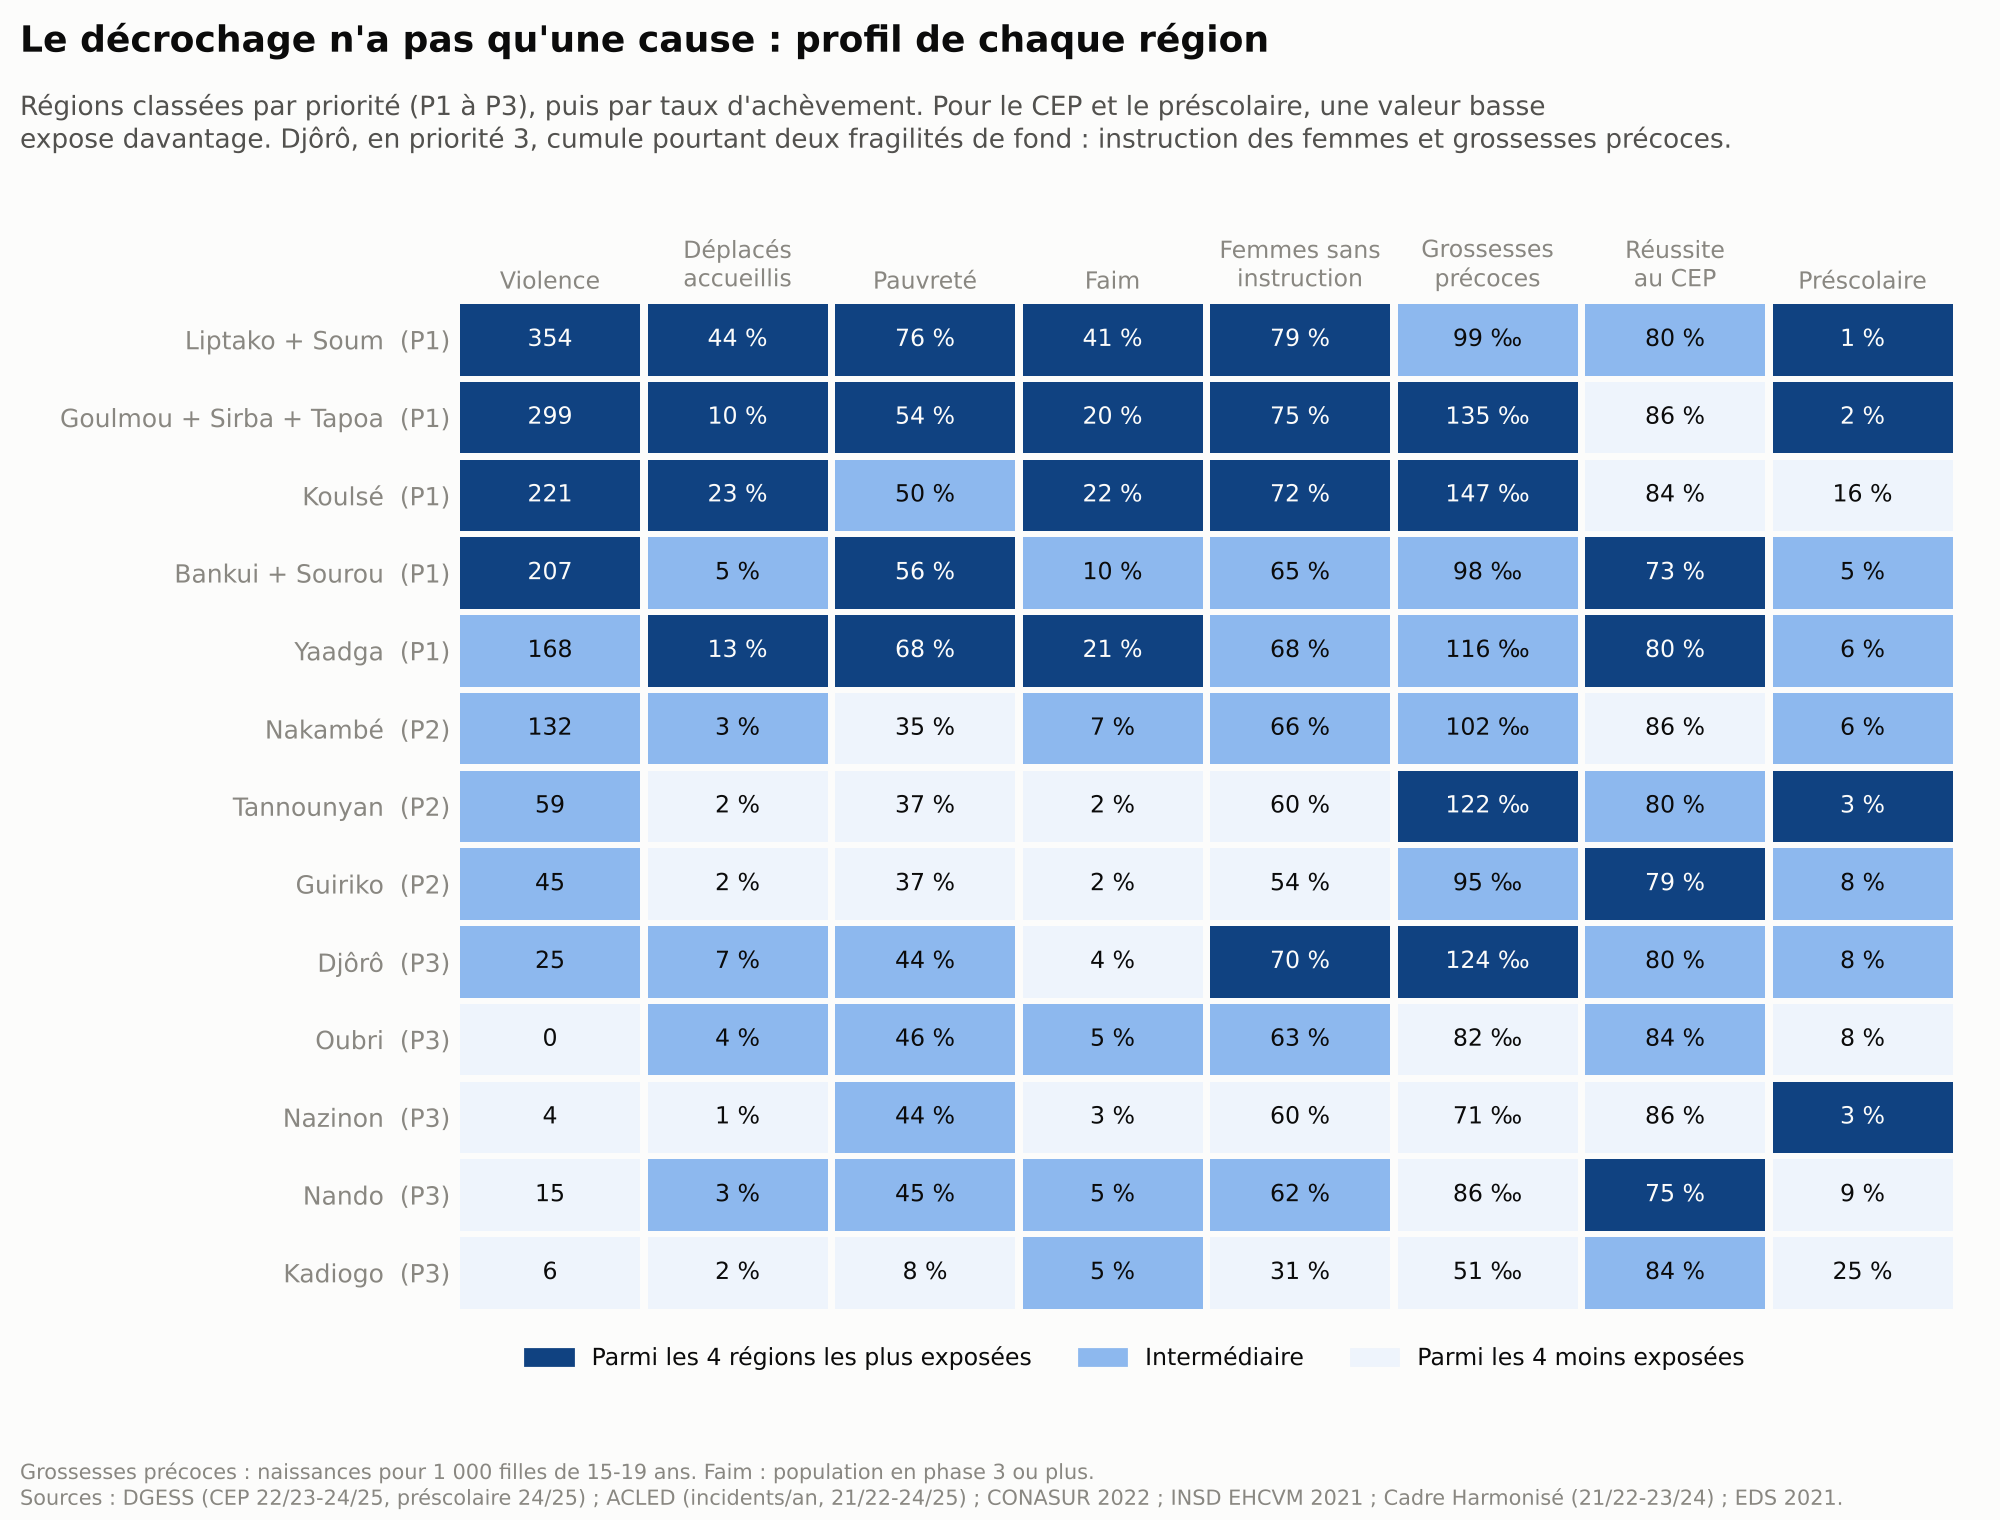
\includegraphics[width=.86\textwidth]{16_profil_facteurs.png}
\caption{Profil des facteurs de fond de chaque région.}\end{figure}

\section{L'outil : un tableau de bord utilisable sans réseau}
L'application s'ouvre sur téléphone comme sur ordinateur. L'accueil présente la carte du score ; un lecteur fait défiler les années de 2020/21 à la prévision 2026/27. Chaque région dispose d'une page : score et décomposition, score année par année jusqu'à la prévision avec les chutes réellement observées, facteur dominant et levier, achèvement, violence, et fiche imprimable.
\begin{figure}[H]\centering
\begin{subfigure}{.235\textwidth}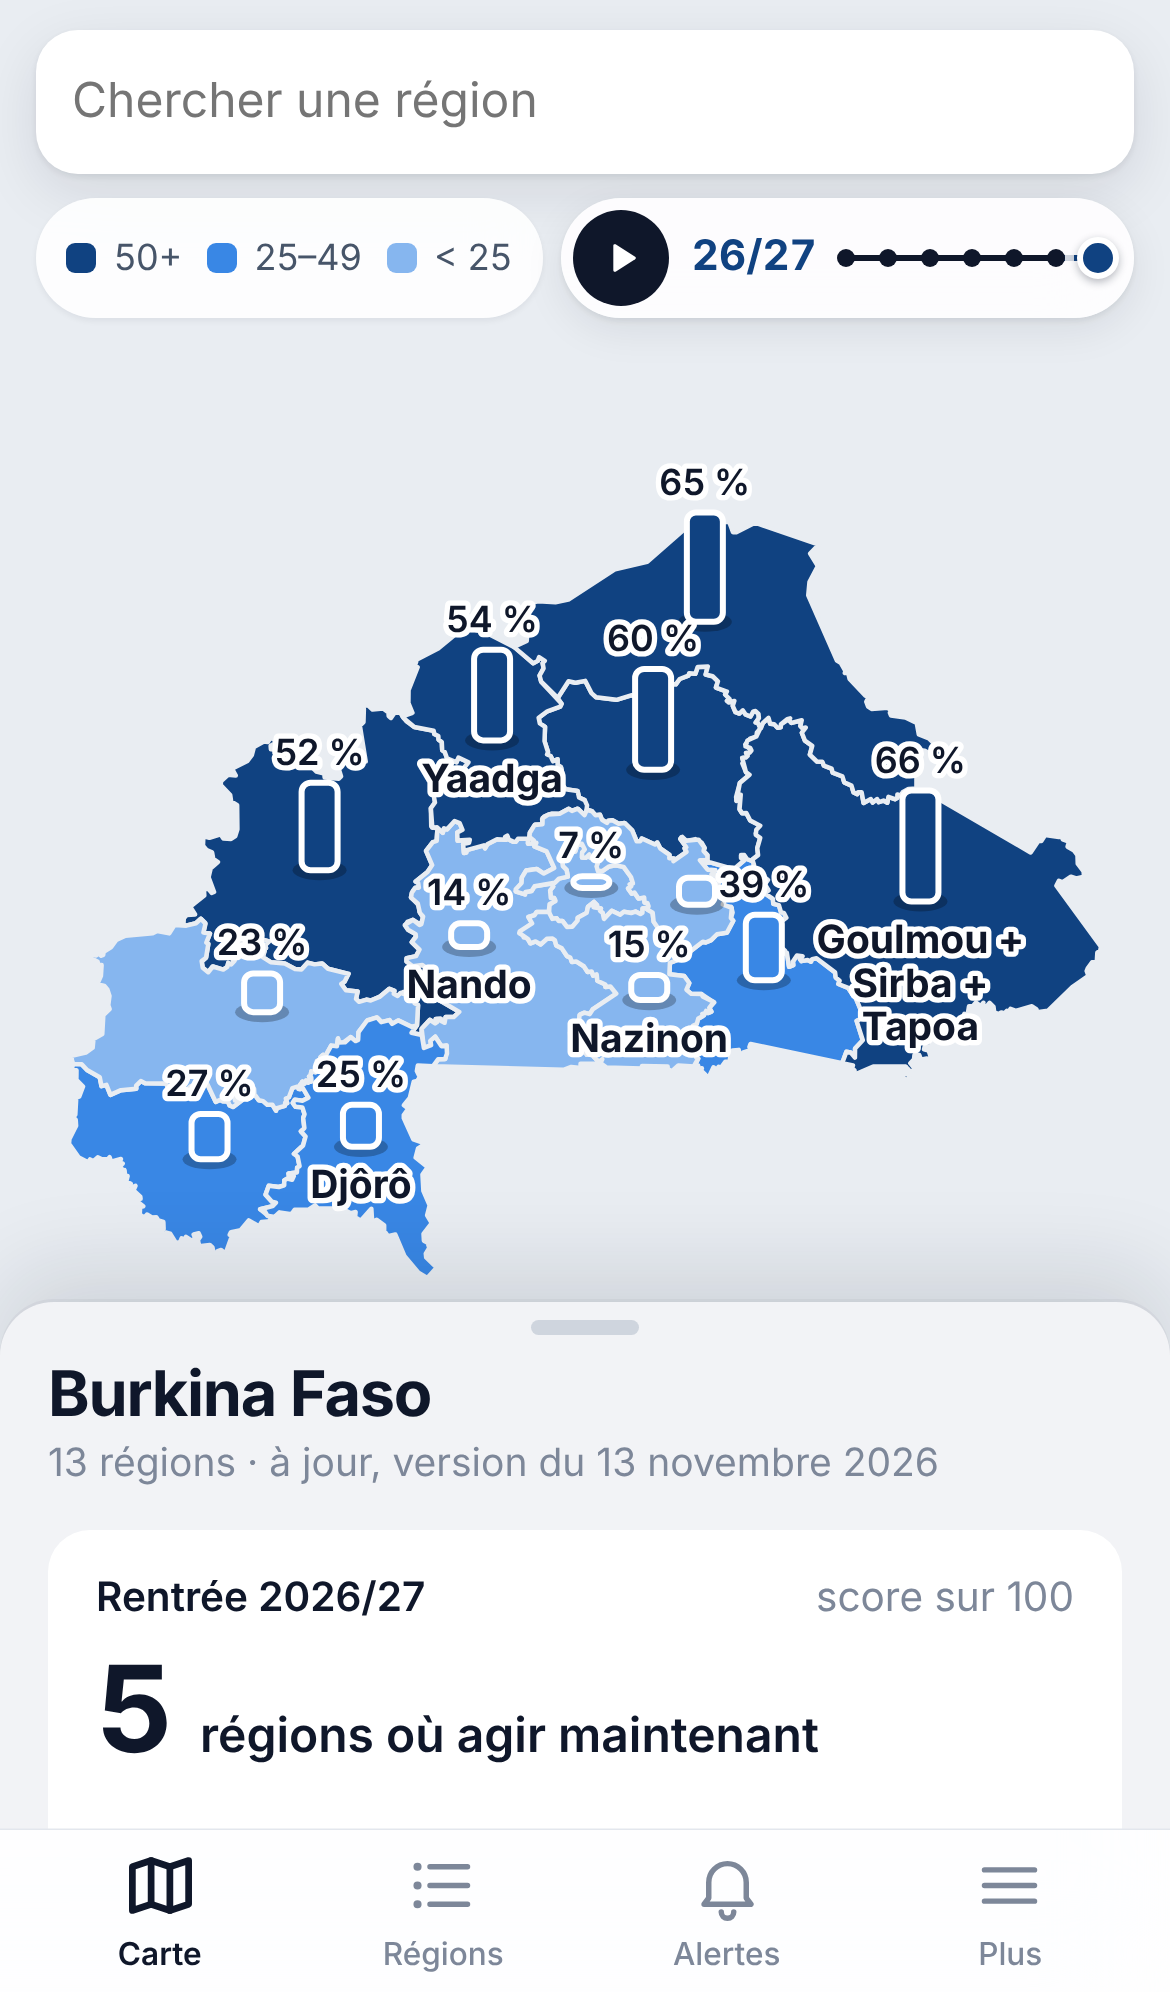
\includegraphics[width=\linewidth]{app_carte.png}\caption{Carte du score.}\end{subfigure}\hfill
\begin{subfigure}{.235\textwidth}
\includegraphics[width=\linewidth]{app_region_score.png}\caption{Score par année.}\end{subfigure}\hfill
\begin{subfigure}{.235\textwidth}
\includegraphics[width=\linewidth]{app_region_action.png}\caption{Sur quoi agir.}\end{subfigure}\hfill
\begin{subfigure}{.235\textwidth}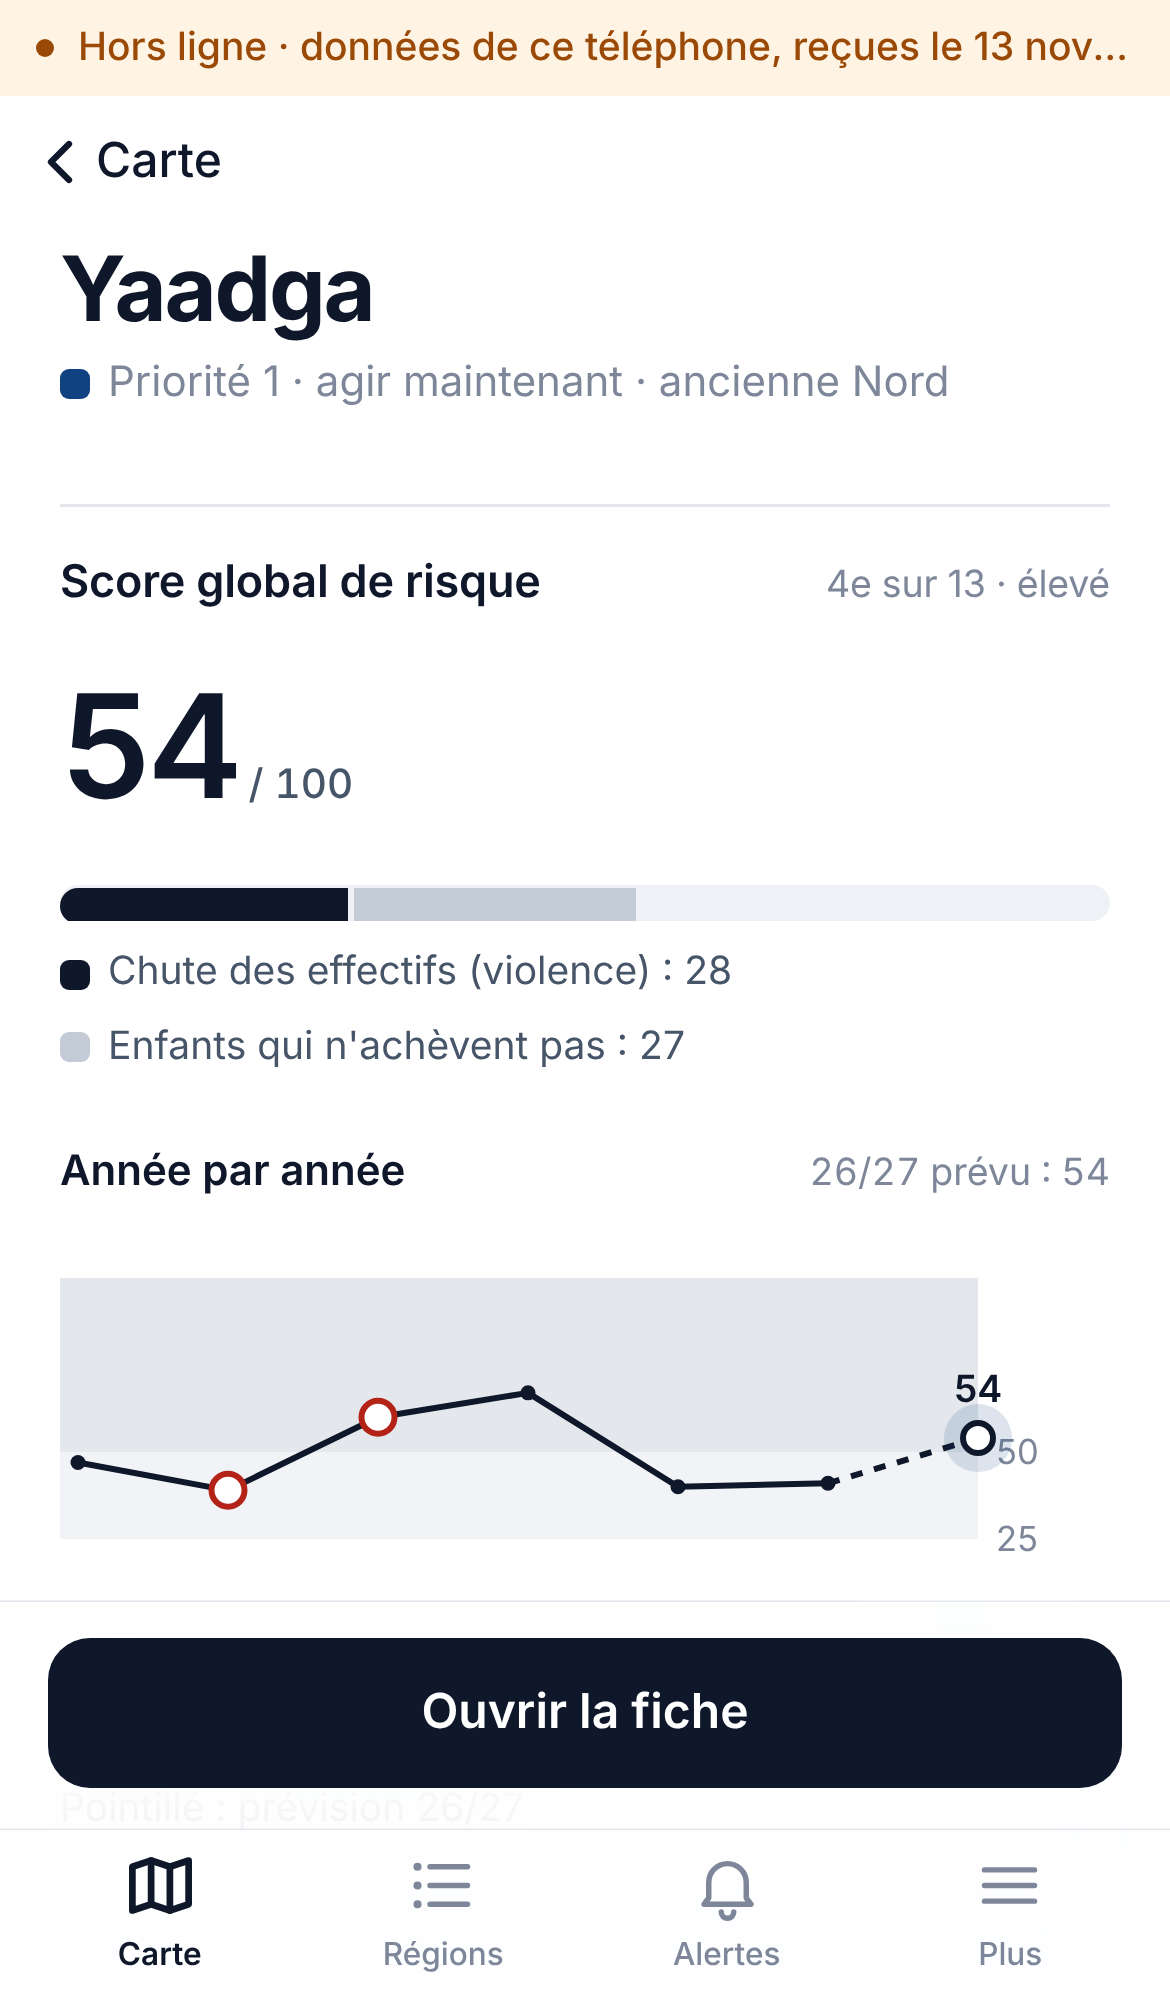
\includegraphics[width=\linewidth]{app_hors_ligne.png}\caption{Serveur arrêté.}\end{subfigure}
\caption{Le tableau de bord sur téléphone. La dernière capture est prise serveur arrêté : l'application s'ouvre et l'indique, avec la date des données.}\end{figure}
Les données sont conservées sur l'appareil ; sans réseau, l'écran l'indique. Le nombre d'écoles ouvertes saisi sur le terrain est enregistré localement, visible immédiatement, puis transmis au retour du réseau, une seule fois. La fiche régionale reste disponible hors ligne. Deux contrôles automatiques vérifient ce fonctionnement à chaque modification, dont l'un serveur réellement arrêté. Les chiffres affichés proviennent d'un fichier unique produit par l'analyse : l'application, les fiches et ce rapport ne peuvent pas se contredire.

\begin{figure}[H]\centering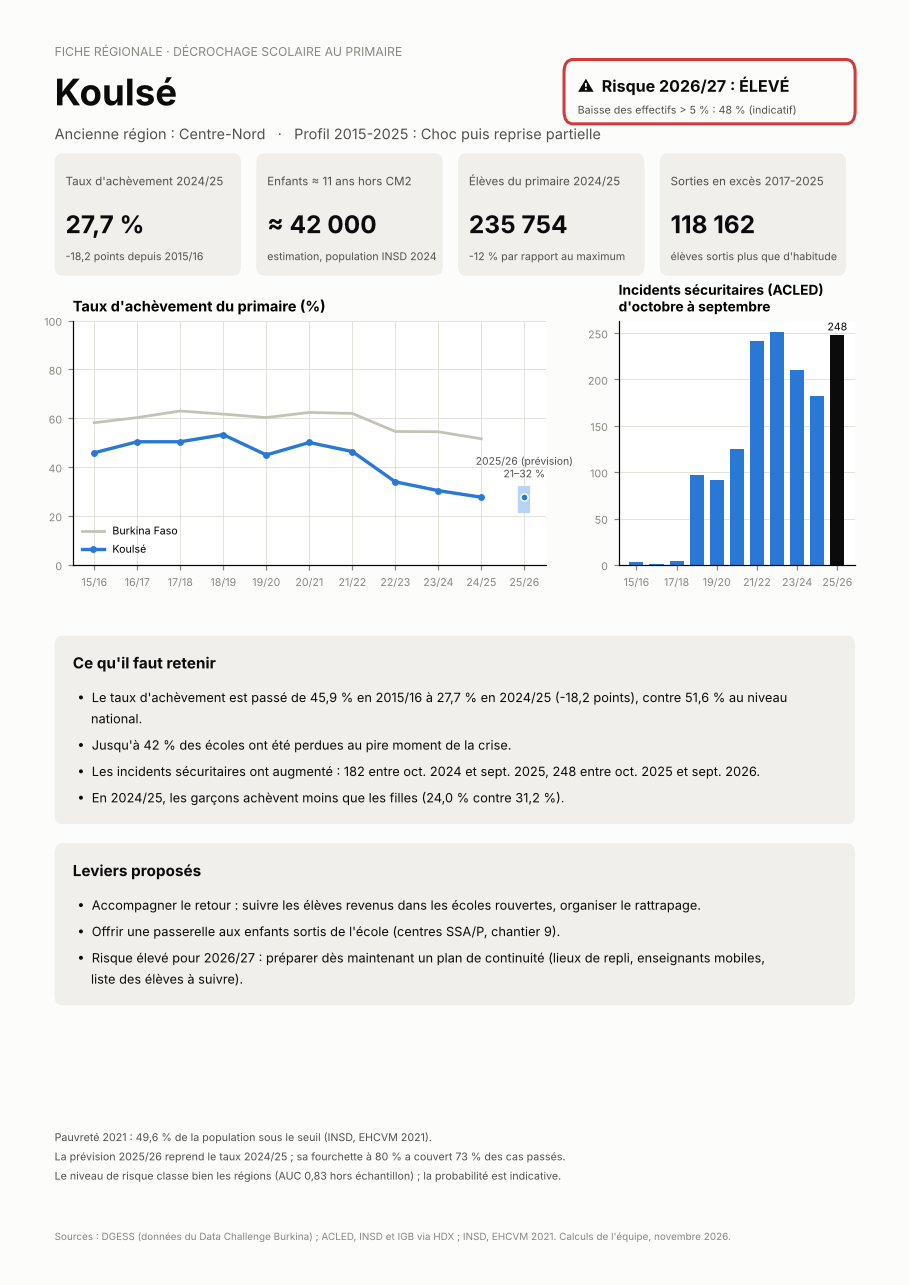
\includegraphics[width=.62\textwidth]{fiche_koulse.png}
\caption{Fiche régionale d'une page (Koulsé, ancien Centre-Nord), destinée à un directeur régional.}\end{figure}

\section{Limites}
\begin{itemize}
\item \textbf{Treize régions}, ni dix-sept ni quarante-sept provinces : c'est le niveau des données du challenge.
\item \textbf{Peu de cas} : 19 fortes baisses pour l'estimation, 14 pour l'évaluation, concentrées sur trois années ; les gains des alertes de septembre et de janvier restent à confirmer.
\item \textbf{L'essentiel du ciblage vient du retard d'achèvement} ; la violence sert surtout à placer en veille une région qui tient encore.
\item \textbf{Les réouvertures ne se prévoient pas} : ce sont des décisions de l'État, d'où la saisie des écoles ouvertes.
\item \textbf{Des taux fragiles} là où les projections de population ignorent les déplacements.
\item \textbf{La faim n'est plus publiée} pour le Burkina après la soudure 2024 ; les facteurs de fond datent de 2021--2022.
\end{itemize}

\section{Perspectives}
\begin{itemize}
\item Alimenter l'outil, dès octobre, avec le nombre d'écoles ouvertes par région, suivi par le ministère : les effectifs de l'année seraient connus avec une erreur divisée par deux, bien avant l'annuaire.
\item Descendre aux quarante-sept provinces dès que les données le permettent ; la violence et la population sont déjà disponibles à ce niveau.
\item Mesurer l'effet des actions en les déployant par vagues, les régions non encore couvertes servant de témoins.
\item Passer à l'école puis à l'élève lorsque le Fichier national des élèves sera généralisé.
\end{itemize}

\section{Reproductibilité}
Le code de chaque étape (nettoyage, transformation, analyse descriptive, modèles, interprétation) est fourni sous forme de cahiers Jupyter exécutés ; relancés, ils redonnent exactement les mêmes résultats. Les vingt et une décisions de méthode sont consignées dans un journal avec ce qu'elles écartent. Seules des données agrégées sont utilisées ; les données brutes d'ACLED ne sont pas redistribuées, conformément à leurs conditions.

\section*{Sources et références}
\small
\begin{itemize}[leftmargin=*]
\item DGESS, Ministère de l'Éducation nationale : données statistiques du préscolaire et du primaire 2015/16--2024/25 (Data Challenge Burkina 2026).
\item ACLED : violence politique et attaques contre les civils, Burkina Faso, par province et par mois (via HDX). IGB, via OCHA : limites administratives v03, 2025. INSD, via UNFPA : population 2024 par province.
\item CILSS/RPCA : Cadre harmonisé. INSD : EHCVM 2021, diagnostic de la pauvreté. INSD/DHS Program : EDS 2021. CONASUR : personnes déplacées internes au 31 décembre 2022. Insecurity Insight : Education in Danger, 2017--2026.
\item Adelman M., Haimovich F., Ham A., Vazquez E. (2018). Predicting school dropout with administrative data. \emph{Education Economics}.
\item IIEP-UNESCO (2024). Données d'éducation en situation d'urgence, Burkina Faso.
\item Kazianga H., Levy D., Linden L., Sloan M. (2013). The effects of girl-friendly schools: evidence from the BRIGHT program in Burkina Faso. \emph{AEJ: Applied Economics}.
\item MEBAPLN (2026). 14 chantiers pour l'école burkinabè à l'horizon 2030.
\item Vazquez E., Haimovich F., Adelman M. (2021). Scalable early warning systems for school dropout prevention. Banque mondiale.
\item Wisner B., Blaikie P., Cannon T., Davis I. (2004). \emph{At Risk}. Routledge.
\end{itemize}
\end{document}
